\documentclass{book}
\usepackage{amsthm,amsmath,amssymb,amsfonts,pstricks}
\usepackage[latin1]{inputenc}
\newcommand{\Z}{\mathbb{Z}}
\usepackage{xparse}
\usepackage{tikz}
\begin{document}
	
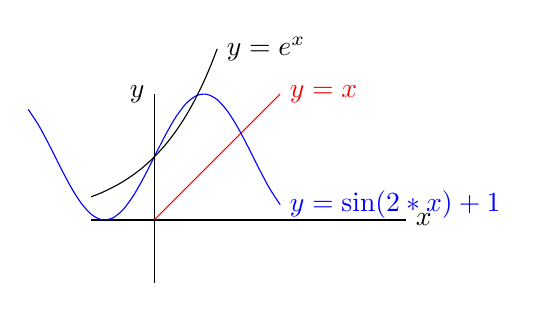
\begin{tikzpicture}[scale=0.8] % Escalamiento de la figura 80%
\draw (-1,0) -- (4,0) node[right] {$x$}; % Ejes
\draw (0,-1) -- (0, 2) node[left] {$y$};
% Dominio: domain = a:b
\draw[smooth, domain = 0:2, color=red] plot (\x,\x)node[right] {$y = x$
};
%\x r indica que x se mide en radianes
\draw[smooth, domain = -2:2, color=blue] plot (\x,{sin(2*\x r)+1})
node[right] {$y = \sin(2*x)+1$};
\draw[smooth, domain = -1:1, color=black] plot (\x,{exp(\x)}) node[right
] {$y = e^x$};
\end{tikzpicture}


\end{document}
